% Lab topology, CVE-2026-53988. Boxes sized by text width (measured labels).
\documentclass[border=5pt,tikz]{standalone}
\usetikzlibrary{arrows.meta,positioning,fit,backgrounds,calc}
\definecolor{labbg}{RGB}{247,250,253}
\definecolor{labframe}{RGB}{110,120,135}
\definecolor{atkfill}{RGB}{253,235,235}
\definecolor{atkline}{RGB}{170,60,60}
\definecolor{vulnfill}{RGB}{255,242,228}
\definecolor{vulnline}{RGB}{190,115,40}
\definecolor{fixfill}{RGB}{232,246,232}
\definecolor{fixline}{RGB}{70,130,70}
\definecolor{netfill}{RGB}{240,244,250}
\begin{document}
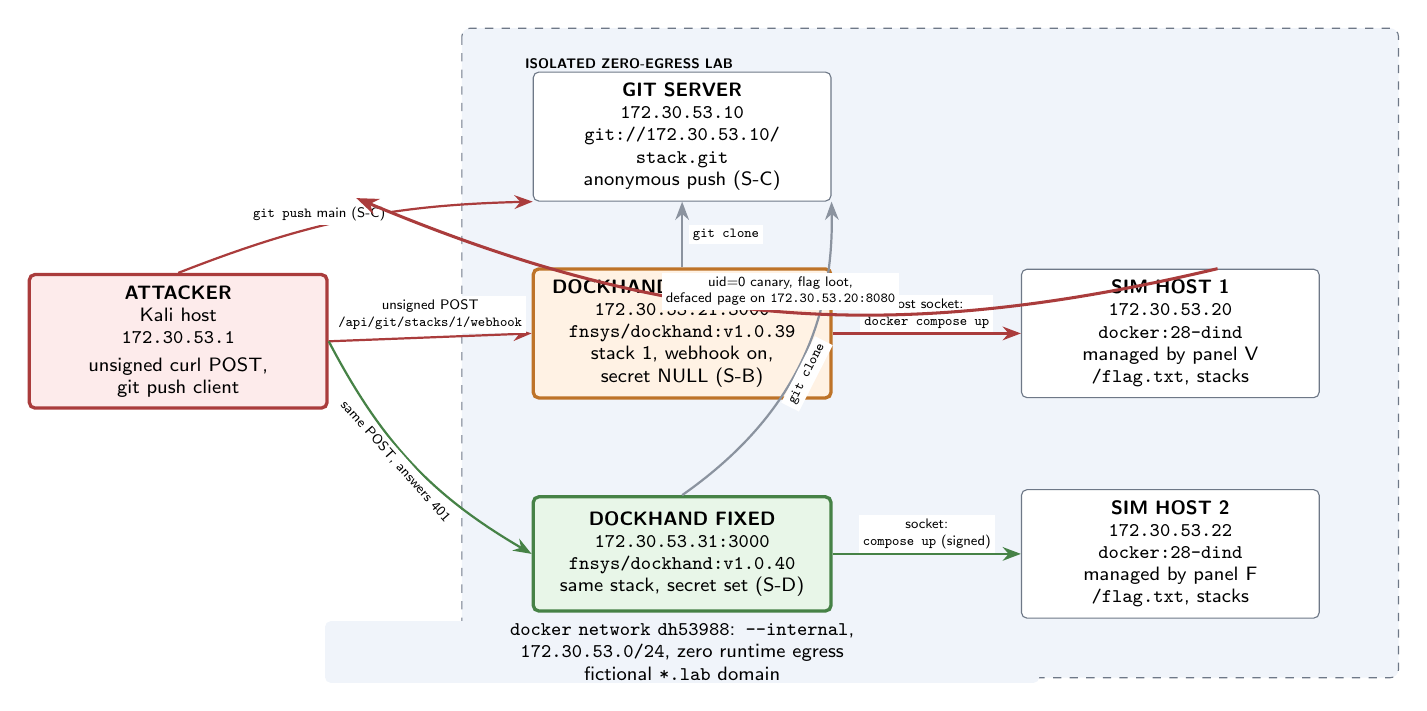
\begin{tikzpicture}[
  >=Stealth, node distance=0cm,
  box/.style={draw=labframe, fill=white, rounded corners=2pt, align=center,
              font=\sffamily\scriptsize, inner sep=4pt, text width=3.3cm,
              minimum height=1.45cm},
  atkbox/.style={box, fill=atkfill, draw=atkline, very thick},
  vuln/.style={box, fill=vulnfill, draw=vulnline, very thick},
  fixed/.style={box, fill=fixfill, draw=fixline, very thick},
  e/.style={->, draw, thick, font=\sffamily\tiny, align=center},
  ered/.style={e, draw=atkline},
  egreen/.style={e, draw=fixline},
  egray/.style={e, draw=labframe!80},
  lbl/.style={font=\sffamily\tiny, align=center, fill=white, inner sep=1.5pt}
]

% ---- attacker
\node[atkbox, text width=3.5cm] (att) at (0,0)
  {\textbf{ATTACKER}\\ Kali host\\ \texttt{172.30.53.1}\\[2pt]
   unsigned curl POST,\\ git push client};

% ---- lab nodes
\node[box, text width=3.5cm] (git) at (6.4,2.6)
  {\textbf{GIT SERVER}\\ \texttt{172.30.53.10}\\
   \texttt{git://\hspace{0pt}172.30.53.10/}\hspace{0pt}\texttt{stack.git}\\
   anonymous push (S-C)};
\node[vuln, text width=3.5cm] (pv) at (6.4,0.1)
  {\textbf{DOCKHAND VULNERABLE}\\ \texttt{172.30.53.21:3000}\\
   \texttt{fnsys/dockhand:}\hspace{0pt}\texttt{v1.0.39}\\
   stack 1, webhook on,\\ secret NULL (S-B)};
\node[fixed, text width=3.5cm] (pf) at (6.4,-2.7)
  {\textbf{DOCKHAND FIXED}\\ \texttt{172.30.53.31:3000}\\
   \texttt{fnsys/dockhand:}\hspace{0pt}\texttt{v1.0.40}\\
   same stack, secret set (S-D)};
\node[box, text width=3.5cm] (h1) at (12.6,0.1)
  {\textbf{SIM HOST 1}\\ \texttt{172.30.53.20}\\
   \texttt{docker:28-dind}\\ managed by panel V\\
   \texttt{/flag.txt}, stacks};
\node[box, text width=3.5cm] (h2) at (12.6,-2.7)
  {\textbf{SIM HOST 2}\\ \texttt{172.30.53.22}\\
   \texttt{docker:28-dind}\\ managed by panel F\\
   \texttt{/flag.txt}, stacks};

% ---- network frame
\begin{scope}[on background layer]
\draw[draw=labframe, dashed, fill=netfill, rounded corners=3pt]
      ($(git.north west)+(-0.9,0.55)$) rectangle ($(h2.south east)+(1.0,-0.75)$);
\node[box, fill=netfill, draw=none, text width=9cm, minimum height=0cm,
      inner sep=1pt] at ($(pf.south)+(0,-0.5)$)
  {\texttt{docker network dh53988}: \texttt{--internal},\\
   \texttt{172.30.53.0/24}, zero runtime egress\\
   fictional \texttt{*.lab} domain};
\end{scope}
\node[font=\sffamily\bfseries\tiny, anchor=north west]
  at ($(git.north west)+(-0.22,0.28)$) {ISOLATED ZERO-EGRESS LAB};

% ---- edges
\draw[ered] (att.east) -- node[lbl, above, yshift=1pt] {unsigned POST\\
  \texttt{/api/git/stacks/1/webhook}} (pv.west);
\draw[egreen] (att.east) to[bend right=16] node[lbl, below, sloped, pos=0.45]
  {same POST, answers 401} (pf.west);
\draw[ered] (att.north) to[bend left=10] node[lbl, above, pos=0.4]
  {\texttt{git push} main (S-C)} (git.south west |- git.south);
\draw[egray] (pv.north) -- node[lbl, right, pos=0.5, xshift=2pt]
  {\texttt{git clone}} (git.south);
\draw[egray] (pf.north) to[bend right=28] node[lbl, below, sloped, pos=0.5]
  {\texttt{git clone}} (git.south east);
\draw[ered] (pv.east) -- node[lbl, above] {host socket:\\
  \texttt{docker compose up}} (h1.west);
\draw[egreen] (pf.east) -- node[lbl, above] {socket:\\
  \texttt{compose up} (signed)} (h2.west);
\draw[ered, line width=1.1pt] (h1.north) ++(0.6,0) to[bend left=18]
  node[lbl, above, pos=0.5] {uid=0 canary, flag loot,\\ defaced page on
  \texttt{172.30.53.20:8080}} ($(att.north east)+(0.35,0.95)$);
\end{tikzpicture}
\end{document}
